\documentclass[11pt]{article}
\usepackage[margin=0.85in]{geometry}
\usepackage{graphicx,booktabs,amsmath,hyperref,xcolor,microtype}
\usepackage[T1]{fontenc}
\usepackage{lmodern}
\definecolor{ink}{HTML}{17283D}
\definecolor{accent}{HTML}{087F8C}
\hypersetup{colorlinks=true,urlcolor=accent,linkcolor=accent,citecolor=accent}
\setlength{\parindent}{0pt}
\setlength{\parskip}{5pt}
\author{James Jean\\\small Independent research}
\date{28 October 2026\\\small GitHub research manuscript; not peer reviewed}

\title{\color{ink}Forecast accuracy is not capacity value\\[4pt]\large A corrected delayed-information evaluation of complaint demand}
\begin{document}\maketitle
\begin{abstract}
An operations team needs a capacity decision, not just a small forecast error. Using six product categories in 102 monthly CFPB snapshots, this study compares three simple rules, four ridge penalties and eight shallow boosting configurations. The last-available-month rule wins forward validation. In the corrected retrospective test, ridge has 16.8\% lower normalized absolute error, yet the paired intervals for three asymmetric capacity-cost scenarios all include zero. Raw RMSE also favors a trailing mean over ridge. The practical recommendation is to retain a simple comparator and evaluate actual operational costs prospectively. A timing audit corrected training-label and normalization cutoffs after the test was first inspected; this paper reports that reused test transparently and makes no new confirmatory claim.
\end{abstract}

\section{The decision}
Shortfalls and unused capacity have different consequences. A model selected on average prediction error may not improve a staffing or queue-management decision. Public complaints provide a useful setting for testing that distinction, but their counts do not measure customer exposure, hours of handling work or all consumer problems. This study allocates abstract capacity units across national product groups; it estimates neither staffing needs nor dollar savings for an employer.

CFPB reporting describes complaint volumes and its API supplies aggregate retrieval \cite{cfpb,api}. The contribution here is an inspectable decision evaluation: a fixed information-delay scenario, a complete small-model search and an explicit comparison between prediction error and asymmetric loss. There is no claim of a new algorithm or an established global literature gap.

\section{Source and information boundaries}
The retained January 2018--June 2026 snapshots reconcile to a separate whole-period query totaling 15,256,569 complaints across 14 source buckets. Only aggregate counts were retained. Six stable labels enter the model: checking/savings, debt collection, money transfers, mortgage, student loans and vehicle loans. Stable labels do not prove stable reporting behavior. A date-boundary probe caught overlapping extraction; the corrected monthly totals reconcile exactly.

At origin $t$, the primary scenario allows counts from $t-2$ and earlier; a sensitivity uses $t-3$. These are assumptions about availability, not historical release vintages. The same cutoff now governs both predictors and training labels. Primary training begins January 2019 and ends November 2022 at the first validation origin. The final fit ends May 2024. The three-month scenario ends each training window one month earlier. Product normalization uses only labels available at the first validation origin.

The original implementation delayed predictors but retained labels and normalization observations too close to the origin. The follow-up audit repaired both. The candidate grid, folds and selection objective were not changed. Because test results had already been inspected, the July 2024--June 2026 rerun is a corrected retrospective evaluation, not an untouched confirmatory test.

\section{Optimization and independent checks}
Three expanding six-month validation folds span January 2023--June 2024. Selection minimizes
\[
  \mathrm{NMAE}=\frac1n\sum_{i=1}^n\frac{|y_i-\hat y_i|}{s_{p(i)}},
\]
where $s_p$ is the frozen training median for product $p$. This is dimensionless, not a percentage error. The candidate set contains last-available, trailing-three-month and seasonal baselines; ridge penalties 0.1, 1, 10 and 100; and eight boosting configurations crossing depth 2/3, learning rate 0.05/0.1 and L2 0/1. Boosting uses 100 iterations and minimum leaf size 12. Preprocessing is fitted inside training folds. The seed is 20261028. Every candidate, fold score and runtime is retained.

MAE, MSE and RMSE are independently recomputed from exported predictions in both raw and normalized units. A separate verifier checks the selected model, training cutoffs and medians. Eight regression tests exercise source corruption, missing/duplicate observations and label-availability boundaries. Two delay scenarios reproduce offline. The selected ridge penalty lies at a grid boundary in each scenario; a finite grid is not proof of a global optimum.

Capacity adds a validation-residual quantile to each point forecast. Shortage-to-surplus ratios 1:1, 3:1 and 9:1 are hypothetical sensitivities, not measured labor costs. Paired monthly losses use a six-month circular-block resampling interval with 2,000 draws. Twenty-four test months provide limited information about uncommon surges.

\section{Results and operational implication}
Primary test NMAE is 1.121 for ridge, 1.348 for the selected last-available baseline and 1.314 for the trailing mean. Ridge improves four of six product groups and worsens two. Its raw RMSE is 5,068 complaints versus 5,037 for the trailing mean; its raw MAE is also worse than that comparator. Thus the model is not best under every error definition.

\begin{table}[ht]\centering
\caption{Normalized capacity losses on the corrected retrospective test. Intervals are conditional block-resampling summaries, not dollars.}
\begin{tabular}{rrrrl}\toprule
Cost ratio & Baseline & Ridge & Difference & 95\% interval\\\midrule
1:1 & 1.347 & 1.135 & -0.212 & [-0.769, 0.111]\\
3:1 & 2.722 & 2.709 & -0.012 & [-0.559, 0.393]\\
9:1 & 6.116 & 6.190 & 0.074 & [-0.596, 0.668]\\
\bottomrule\end{tabular}\end{table}

Every interval includes zero. This does not establish equivalence; it means the observed predictive advantage is insufficient evidence to replace the capacity rule. The three-month scenario selects ridge penalty 100 and likewise leaves the capacity-value conclusion uncertain.

\begin{figure}[ht]\centering
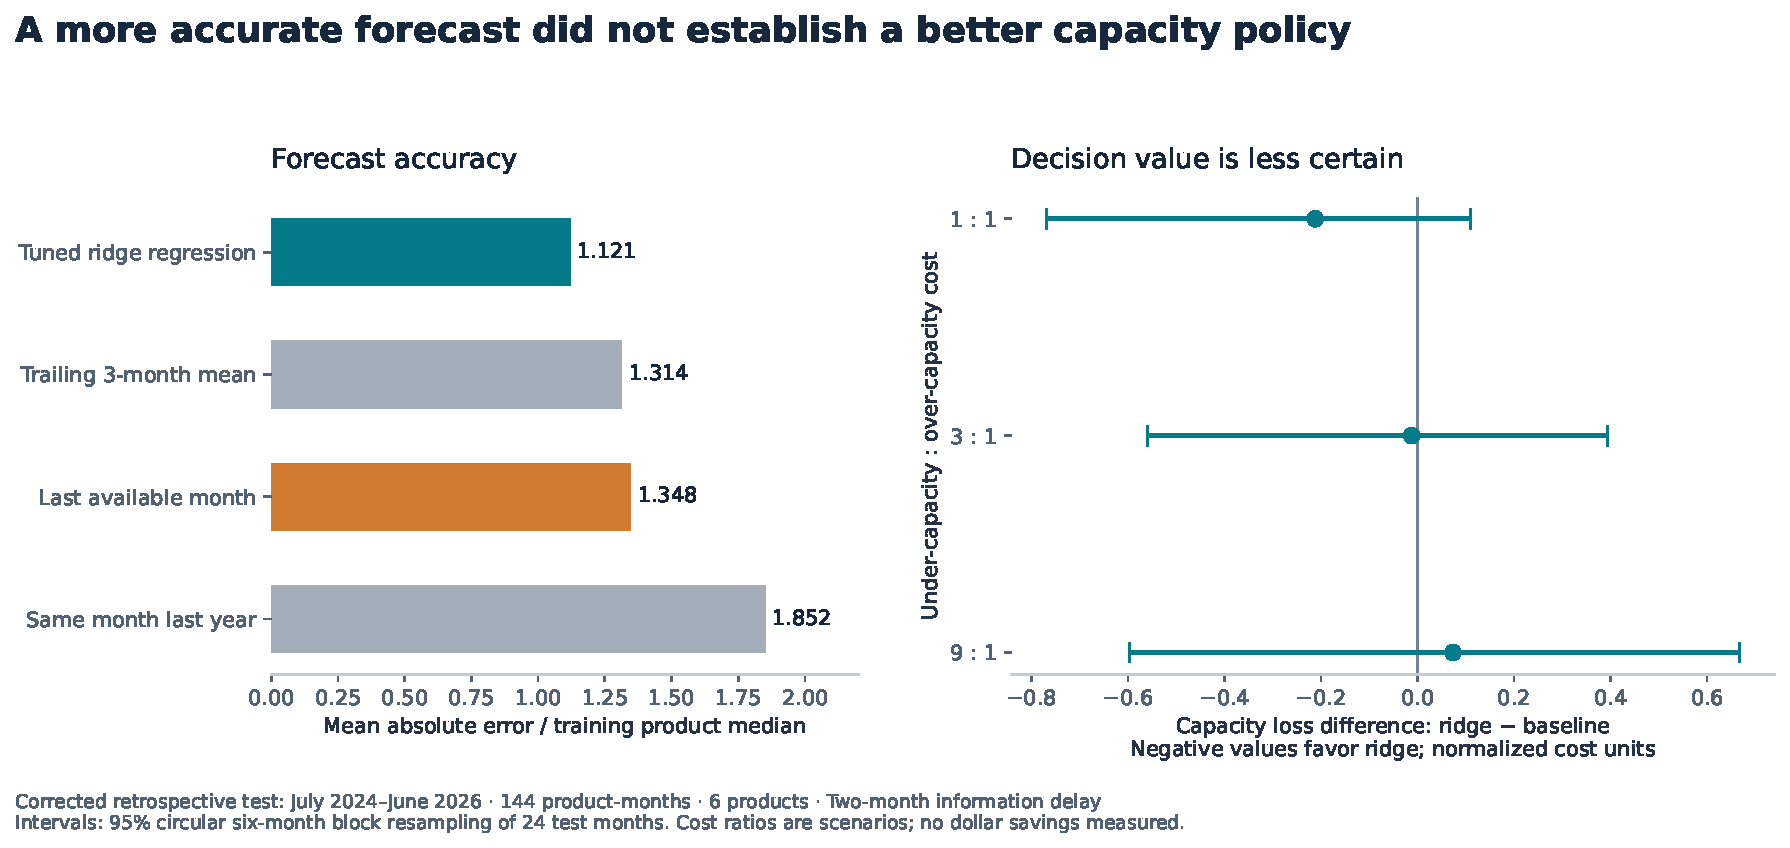
\includegraphics[width=\linewidth]{images/forecast-and-decision.pdf}
\caption{Prediction and decision metrics answer different questions. The full source, search table and numeric evidence accompany the public code.}
\end{figure}

\section{Limitations and next experiment}
Final snapshots can include revisions unavailable at the original forecast date. Publication and reporting behavior affect counts. Renamed categories are omitted, residual calibration pools products, the test horizon is short and backlog carryover is not modeled. The corrected test cannot provide a new confirmatory claim. A useful next experiment would save release vintages and use institution-specific workload, service times and agreed shortage costs in a prospective shadow evaluation. No deployment, causal effect or realized business benefit is claimed.

\section*{Reproducibility}
Code, eligible aggregate snapshots, source hashes, complete candidate results, prediction exports, independent checks and figures are public at \href{https://github.com/S3R3Bii/complaint-capacity-forecasting}{the public research repository}. This research manuscript is shared with the reproducible GitHub package and has not been peer reviewed. AI assisted coding and drafting; retained calculations and checks support the numeric claims.

\begin{thebibliography}{9}
\bibitem{cfpb} Consumer Financial Protection Bureau. \emph{Consumer Complaint Database}. Accessed 28 October 2026. \url{https://www.consumerfinance.gov/data-research/consumer-complaints/}.
\bibitem{api} Consumer Financial Protection Bureau. \emph{Consumer Complaint Database API}. \url{https://cfpb.github.io/api/ccdb/}.
\end{thebibliography}\end{document}
